\documentclass[../main.tex]{subfiles}

\begin{document}
    \subsection{プロセッサ名}
        この演習で設計したプロセッサの名前を,「grapy 」と名付けた。
        その由来は、最近ぶどうにハマってしまって、「grape 」だと独特はなく、「grapy 」にした。
        それぐらいの気持ちでこの設計演習に取り組んだということを伝えたい。

    \subsection{命令セット}
        本プロセッサがサポートするRISCV 32Iの命令を表\ref{table:instructions}に示す。
        命令は全て32bitの幅長であり、それぞれある命令形式に従っている。
        命令形式には、R 形式、I 形式、S 形式、B 形式の4種類がある。
        また命令形式は図\ref{fig:inst}に示してある。
        \begin{figure}[h]
            \centering
            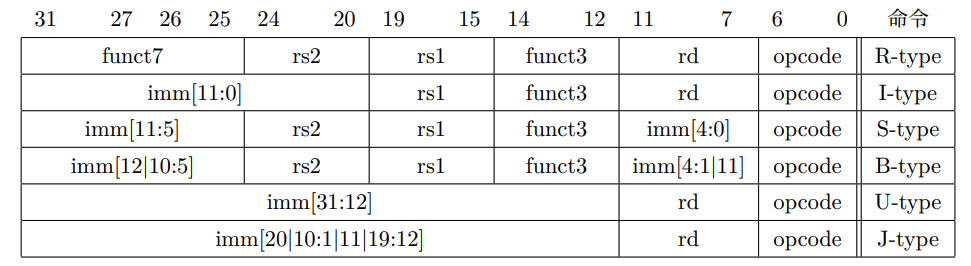
\includegraphics[width = 1.5\columnwidth]{../images/insts.png}
            \caption{命令形式}
            \label{fig:inst}
        \end{figure}
        \subfile{./insts.tex}

    \subsection{外部インタフェース}
    本プロセッサは5段パイプライン処理を導入することため、命令フェッチとデータアクセスの資源競合存在する。
    このような状態を避けるため、ハードウェア的なアプローチをとり、
    命令用メモリおよびデータ用メモリに対して同時にアクセス可能である。
    また,命令およびデータを扱うとき、幅長は全て32bitで,メモリはバイト単位で格納されている。
    図\ref{fig:processor}に外部インターフェイスとプロセッサの接続を示す。
    ここで,信号名の末尾に付いている$\#$は,信号線が負論理(Low でアクティブ)であることを意味する。

    \begin{figure}[h]
        \centering
        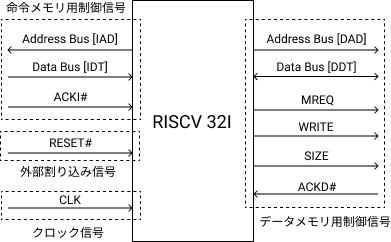
\includegraphics[width = 1.3\columnwidth]{../images/cpu.png}
        \caption{プロセッサの外部インタフェース}
        \label{fig:processor}
    \end{figure}

\end{document}
